\hypertarget{(chap:capitolo6)}{}
\chapter{Risultati sperimentali}
In questo capitolo andremo a vedere i risultati sperimentali per ogni metodo.
\section{Risultati preprocessing matrici grezze}
Nelle sezione successive andremo a vedere i risultati delle valutazioni di ciascun modello rispetto la metrica $AUC$ e la $NDCG$ con $k\in \{5, 10, 25, 100\}$, in particolare la metrica che riteniamo sia più significativa è la seconda in quanto si basa sul ranking degli item nella lista $TopN$. \\
Per i confronti abbiamo scelto di usare $NDCG$ con $k=25$. Nei seguenti grafici

\subsection{Risultati base}
In questa sezione andremo a vedere i risultati del modello MostPop e del VAECF, che verranno utilizzati come bound per valutare quelli succcessivi. 

\subsubsection{MostPop}
Come detto il modello MostPop restituisce per ogni user la stessa lista di item più popolari.
Andiamo a vedere i risultati per dataset sul validation set:\\

\begin{tabular}{|l|c|cccc|}
    \toprule
    $dataset$ &    $AUC$ &  $NDCG@10$ & $NDCG@100$  & $NDCG@25$ & $NDCG@5$  \\
    \midrule
    macchine & 0.7644 & 0.1263 &   0.2414 &  0.1647 & 0.0920 \\
    ricambi  & 0.3427 &  0.0299 &   0.0732 &  0.0358 & 0.0000 \\
    totale  & 0.2810 &  0.0733 &   0.0811 &  0.0627 & 0.0360 \\

\bottomrule
\end{tabular}\\

Useremo questi risultati come bound per quelli degli altri modelli (MF, UserKnn), nel caso in cui questi siano migliori si procederà al tuning dei parametri e al calcolo finale dei risultati sul test set.\\
Quelli riportati qui di seguito sono i risultati del MostPop sul test set.\\

\begin{tabular}{|l|c|cccc|}
    \toprule
    $dataset$ &    $AUC$ &  $NDCG@10$ & $NDCG@100$  & $NDCG@25$ & $NDCG@5$  \\
    \midrule
    macchine & 0.7897 &  0.1364 &   0.2610 &  0.1875 & 0.1001 \\
    ricambi  & 0.3924 &  0.0753 &   0.1365 &  0.0793 & 0.0619 \\
    totale  & 0.3101 &  0.0807 &   0.1281 &  0.0866 & 0.0944 \\

\bottomrule
\end{tabular}

\subsubsection{VAECF}
Il modello VAECF è un modello che funziona su rating impliciti, la fase preliminare ha richiesto il tuning dei parametri riportati di seguito:
\begin{itemize}
    \item $n_{int}$ è la dimensione della rappresentazione latente interna, i possibili valori sono $\{5,10,15,20,50\}$;
    \item $n_{hid}$ è il numero di neuroni del layer dell'encoder e del decoder, i valori possibili sono $\{10,20,30,50,100,200\}$;
    \item $f_{act}$ è la funzione di attivazione applicata nei layer nascosti, che può essere una delle seguenti $\{sigmoid, tanh, elu, relu, relu6\}$.
\end{itemize}
\begin{minipage}[H]{0.45\textwidth}
    \begin{tabular}{|l|ccc|}
        \toprule
        $dataset$ &    $n_{int}$ &  $n_{hid}$ & $act\_f$ \\
        \midrule
        macchine & 5 & 30 & relu \\
        ricambi  &	5 & 30 & sigmoid\\
        totale  & 5 & 30 & sigmoid\\
    \bottomrule
    \end{tabular}\\
\end{minipage}
\begin{minipage}[H]{0.55\textwidth}
    Il tuning dei parametri ha portato a considerare tutte le possibili combinazioni dei parametri sopra citati, andiamo a vedere per ogni dataset quali parametri hanno restituito sul validation set i risultati migliori.
\end{minipage}\\

Andiamo a vedere i risultati per dataset sul validation set dopo il tuning dei parametri:\\

\begin{tabular}{|l|c|cccc|}
    \toprule
    $dataset$ &    $AUC$ &  $NDCG@10$ & $NDCG@100$  & $NDCG@25$ & $NDCG@5$  \\
    \midrule
    macchine & 0.8201 & 0.1768 & 0.3032 & 0.2282 & 0.1325 \\
    ricambi & 0.4773 & 0.0452 & 0.1052 & 0.0643 & 0.0506 \\
    totale  & 0.4190 & 0.0980 & 0.0941 & 0.0741 & 0.1208 \\
\bottomrule
\end{tabular}\\

Dato che i risultati della tabella precedente sono quelli del validation set su un modello con parametri ottimizzati, non possiamo direttamente usarli per il confronto con 

Vediamo i risultati del modello validato sul test set:\\

\begin{tabular}{|l|c|cccc|}
    \toprule
    $dataset$ &    $AUC$ &  $NDCG@10$ & $NDCG@100$  & $NDCG@25$ & $NDCG@5$  \\
    \midrule
    macchine & 0.8269 &  0.1948 &   0.3301 &  0.2487 & 0.1473 \\
    ricambi  & 0.4930 &  0.0919 &   0.1401 &  0.1075 & 0.0801 \\
    totale  & 0.4343 &  0.0874 &   0.1398 &  0.0964 & 0.0988 \\

\bottomrule
\end{tabular}

\subsection{Risultati MF e UserKnn}
In questa sezione andremo a vedere per ogni tecnica di preprocessing adottata sulle matrici grezze i risultati ottenuti.
La valutazione si è divisa in due fasi: 
\begin{enumerate}
    \item preliminare: confrontiamo i risultati dei modelli (MF, UserKnn) con parametri di default sulle matrici dei rating, con il risultato bound dato dal MostPop;
    \item avanzata: dopo aver effettuato il tuning sui parametri dei modelli con le matrici rimanenti, si confrontano con il bound dato dal VAECF. 
\end{enumerate} 
Cominceremo prima con la tecnica basata su min-max, poi con quella ordered-based per concludere infine con quella basata sui prodotti totali. 
Spesso si farà riferimenti ai risultati dei modelli, intendendo il risultato dato dei modelli basato sulle diverse matrici dei rating.

\subsubsection{Normalizzazione min-max}
Come spiegato nel capitolo dedicato alle tecniche ora andremo ad osservare i risultati rispetto diversi gruppi di triplette.\\

\paragraph{Gruppo globale}\mbox{} \\
In questa sezione vedremo la normalizzazione min-max applicata al gruppo globale, ossia quello contenente tutte le triplette.
Nella tabella sottostante possiamo vedere sulle righe i dataset (macchine, ricambi, totale), mentre sulle righe possiamo vedere le \textit{espressioni d'interesse}. Ciascun grafico poi mostra sulle ascisse la $scale$ della matrice dei rating e sulle ordinate il risultato ottenuto da tale matrice rispetto la metrica $NDCG@25$. \\
La linea tratteggiata blu rappresenta il risultato del modello MostPop che viene usato come bound.
In questo grafico composto per ogni valore della scala vengono riportati quattro puntini, per questa tecnica ogni matrice dei rating è stata tenuta sia in versione continua che in versione intera, a queste due matrici vengono applicati i due modelli, da cui vengono fuori quindi quattro risultati, quelli di colore blu sono i risultati forniti dal modello MF, mentre quelli arancioni quelli del modello UserKnn.

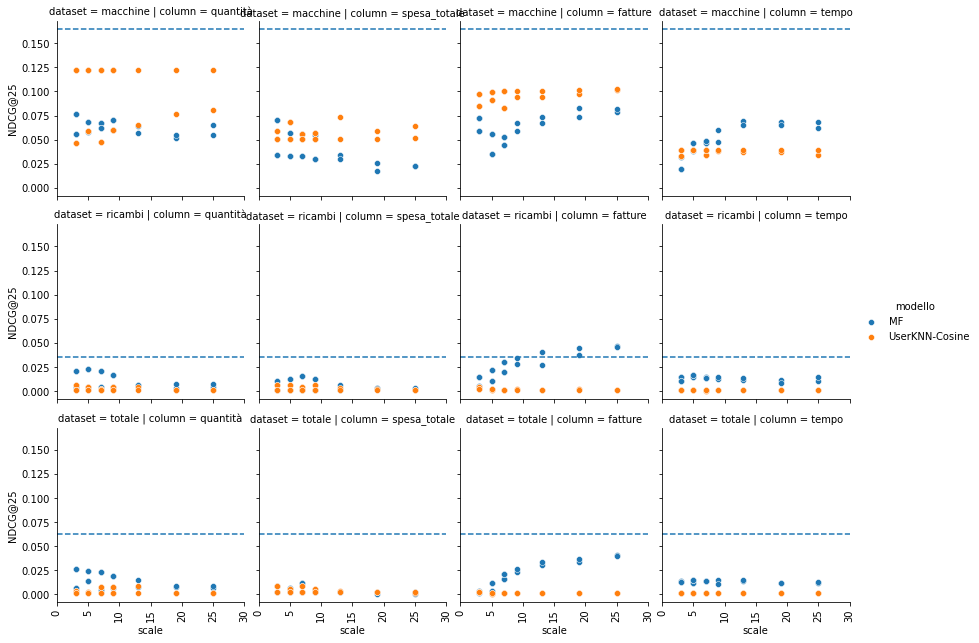
\includegraphics[width=16cm]{figures/risultati_minmax_globale.png}

Diamo un commento ai risultati per ogni tipo di dataset:\\
\subparagraph{Macchine}\mbox{} \\

Per il seguente dataset non presenta alcun risultato che superi il livello di sbarramento, possiamo dire però che le espressioni d'interesse quantità e numero di fatture risultano essere migliori rispetto le restanti. Notiamo anche che la scala sembra avere effetto sui risultati anche se questi possiamo dire che si trovino circa nello stesso intervallo di valori della metrica. Il modello UserKnn sembra funzionare meglio rispetto MF per tutte le espressioni d'interesse tranne che per la recentezza. Per ogni valore della scala si possono vedere due pallini per ciascun colore, questo perché c'è una versione della matrice continua e una intera. Vediamo di seguito come si comportano:

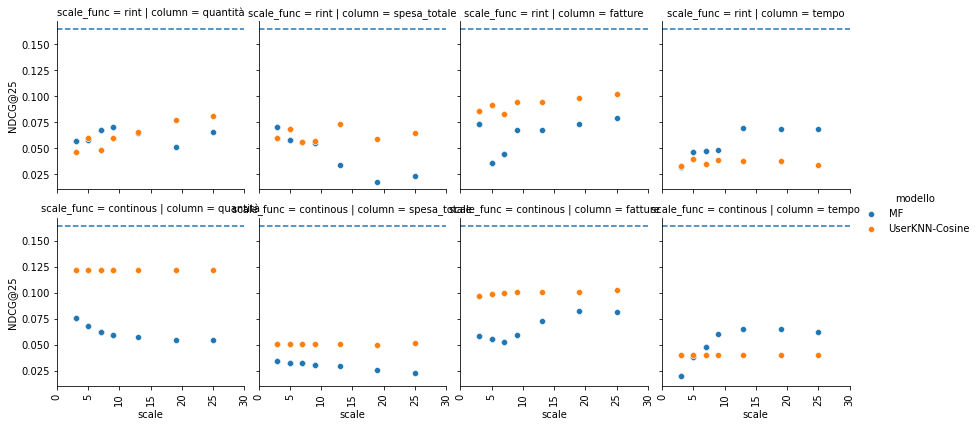
\includegraphics[width=16cm]{figures/scale_func_minmax_glob_macchine.png}

La prima riga utilizza le matrici intere mentre la seconda quelle continue, come possiamo vedere i risultati della versione continua sono più lineari rispetto gli altri. Nonostante ciò possisamo dire che i risultati siano tendenzialmente simili, a parte che per la prima colonna (quantità) dove il modello UserKnn migliora di molto con la versione della matrice continua. In generale questo varà per tutti i grafici che andremo a vedere dove viene applicato min-max.

\subparagraph{Ricambi}\mbox{} \\
Per questo tipo di dataset abbiamo un'espressione d'interesse che ha superato la soglia di sbarramento, quella del numero di fatture, potrebbe essere che questa abbia una distribuzione dei valori di partenza più piatta rispetto le controparti (quantità, spesa totale), in quanto ciascun prodotto ha una quantità e un costo diverso, mentre il numero di fatture è più legato alla frequenza d'acquisto.
Per quanto riguarda la scala sembra esserci una tendenza per l'espressione numero di fatture a migliorare all'aumentare del valore massimo di scala.
Le affermazioni riportate precedentemente per quanto riguarda matrici intere e continue valgono anche qui.

\subparagraph{Totale}\mbox{} \\
In questo tipo di dataset non abbiamo valutazioni che superino la soglia, la tendenza dei dati richiama molto quella del dataset tipo ricambi, non a caso il totale è formato per buona parte dalle triplette dei ricambi. 

\paragraph{Gruppi user-based}\mbox{} \\
In questa sezione vedremo la normalizzazione min-max applicata al gruppo user-based, ossia quello dove ciascun gruppo contiene solo le triplette di un singolo user. Il grafico composto di seguito possiede la stessa disposizione di quello del paragrafo precedente.

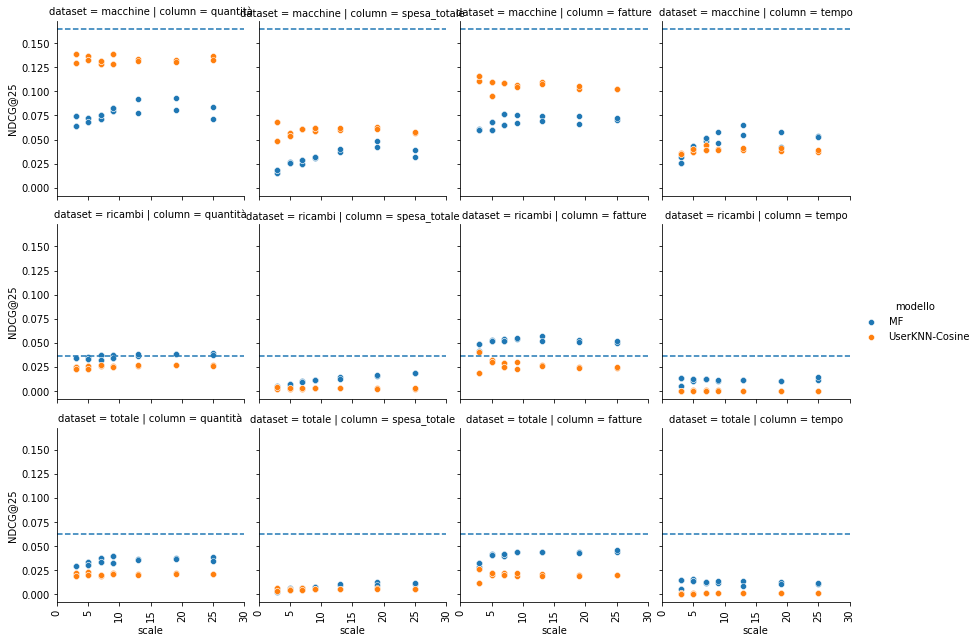
\includegraphics[width=16cm]{figures/risultati_minmax_singolo.png}
Notiamo come ci siano un leggero miglioramento dei risultati rispetto il gruppo globale, vediamo singolarmente ciascun tipo di dataset.

\subparagraph{Macchine}\mbox{} \\
Possiamo notare che i risultati siano migliorati rispetto i precedenti, ma non hanno ancora superato la soglia per passare alla fase avanzata, il modello UserKnn fuziona molto bene rispetto MF, come in precedenza le espressioni d'interesse quantità e numero di fatture funzionano meglio delle altre due. Anche qui si nota una tendenza della scala ad avere risultati migliori con valori intorno a 25. 

\subparagraph{Ricambi}\mbox{} \\
Con questo gruppo possiamo notare come l'espressione numero di fatture rispetto il tipo dataset ricambi sia molto migliorata e ora quasi tutte i risultati con modello MF sono sopra la soglia critica. Inoltre anche la quantità si trova in alcuni risultati intorno al valore soglia. In generale comunque i risultati sembrano in generale migliori del gruppo globale.

\subparagraph{Totale}\mbox{} \\
Non abbiamo alcun risultato ancora sopra la soglia, anche se i risultati sembrano un po' meglio dei precedenti.

\paragraph{Gruppo user-category-based}
Ora andremo a vedere la normalizzazione min-max applicata però al gruppo user-category-based, dove le triplette vengono divise per user e per categoria.
Le categorie utilizzate sono quelle della gerarchia prodotto e del gruppo merceologico. Vediamo ora per ogni tipo di dataset i risultati sperimentali.


\subsubsection{Tecnica ordered-based}

\paragraph{Gruppo globale}\mbox{} \\
In questa sezione vedremo la tacnica di preprocessing ordered-based applicata al gruppo globale, ossia quello contenente tutte le triplette.
Nella tabella sottostante possiamo vedere sulle righe i dataset (macchine, ricambi, totale), mentre sulle righe possiamo vedere le \textit{espressioni d'intresse}. Ciascun grafico poi mostra sulle ascisse la $scale$ della matrice dei rating e sulle ordinate il risultato ottenuto da tale matrice rispetto la metrica $NDCG@25$. La linea tratteggiata blu rappresenta il risultato del modello MostPop che viene usato come bound.
Inoltre i puntini di colore blu rappresentano i risultati forniti dal modello MF, mentre quelli arancioni dallo UserKnn.

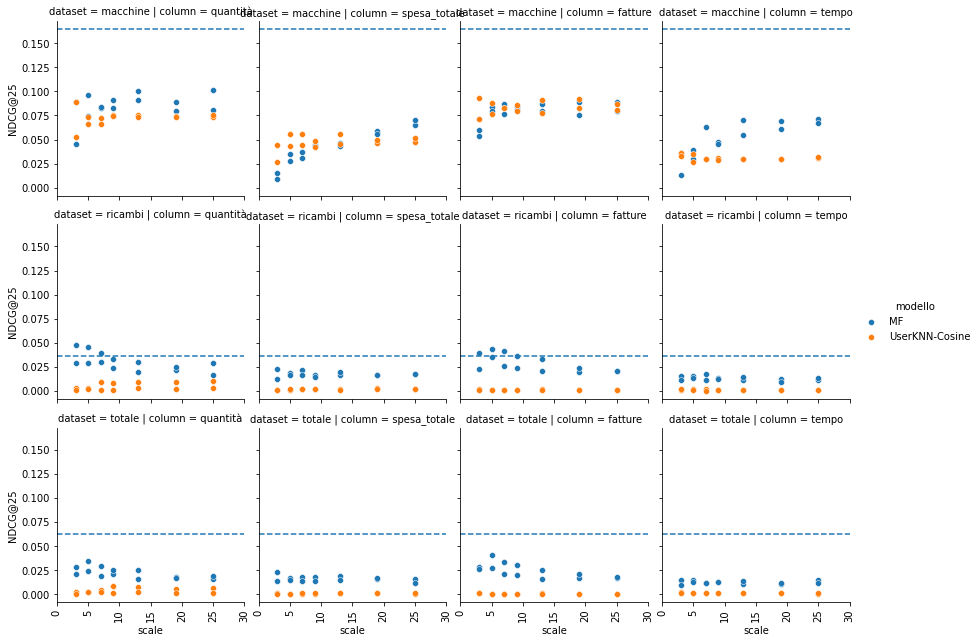
\includegraphics[width=16cm]{figures/risultati_ordered_globale.png}

Nella tabella di grafici sopra riportati possiamo vedere sulle righe i dataset (macchine, ricambi, totale), mentre sulle colonne possiamo vedere le espressioni d'interesse (quantità, )

\paragraph{Gruppi user-based}\mbox{} \\
Di seguito possiamo vedere i risultati relativi la tecnica ordered-based su gruppi di triplette appartenenti allo stesso user.\\
I grafici sono organizzati come segue: sulle righe i dataset (macchine, ricambi, totale), mentre sulle righe possiamo vedere le \textit{espressioni d'intresse}. Ciascun grafico poi mostra sulle ascisse la $scale$ della matrice dei rating e sulle ordinate il risultato ottenuto da tale matrice rispetto la metrica $NDCG@25$. La linea tratteggiata blu rappresenta il risultato del modello MostPop che viene usato come bound.
Inoltre i puntini di colore blu rappresentano i risultati forniti dal modello MF, mentre quelli arancioni dallo UserKnn.\\

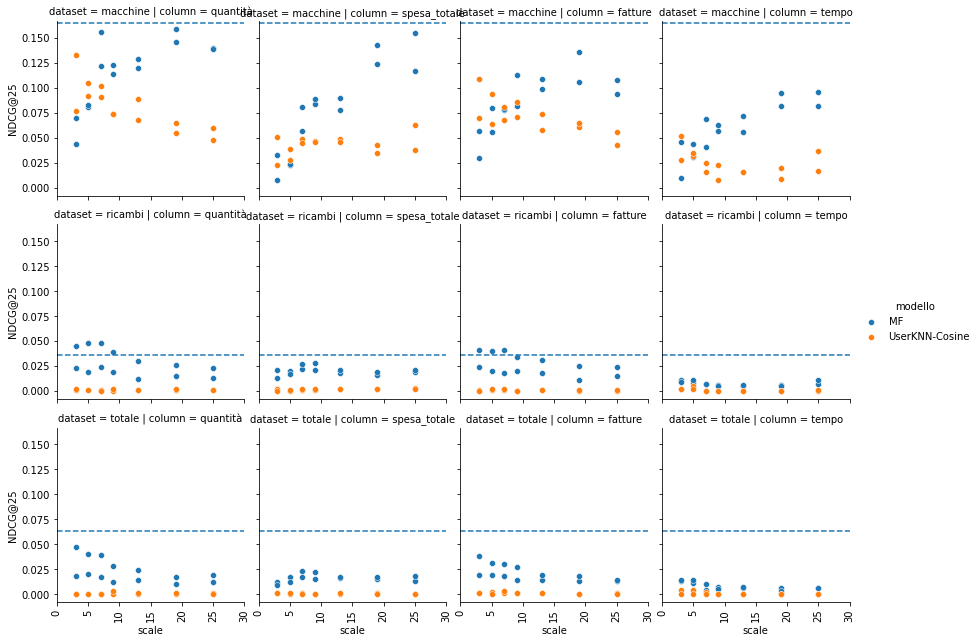
\includegraphics[width=16cm]{figures/risultati_ordered_singolo.png}

Possiamo vedere come il metodo non funzioni se non per alcuni risultati nell'incrocio (ricambi,quantità) che superano di poco il livello bound.

\paragraph{Gruppo user-category-based}\mbox{} \\
\begin{comment}
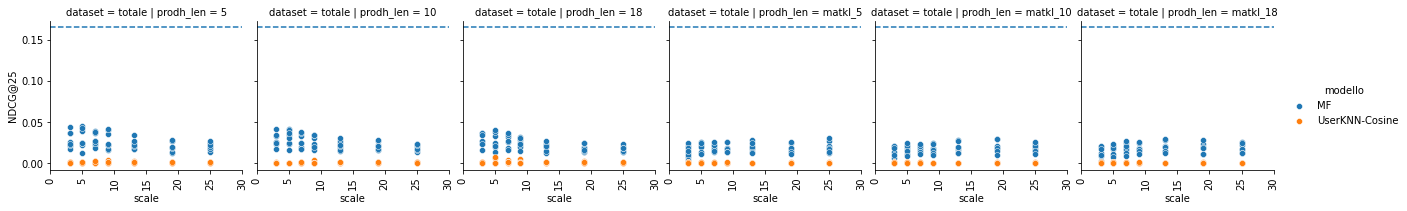
\includegraphics[width=16cm]{figures/risultati_ordered_categoria.png}
\end{comment}
\subsubsection{Tecnica product-based}

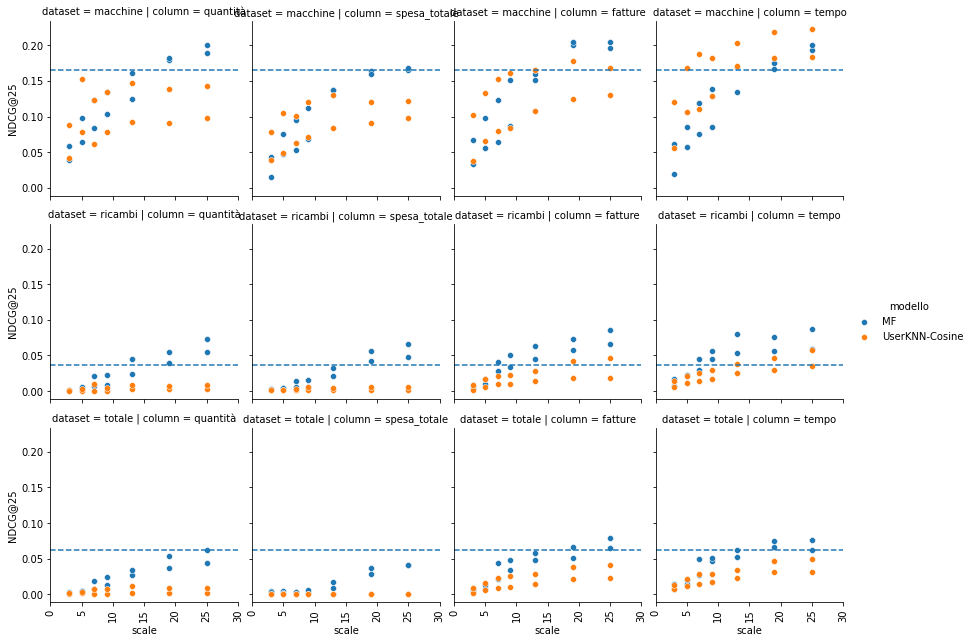
\includegraphics[width=16cm]{figures/prodotto.png}

\section{Risultati matrici grezze combinate}
Vediamo di seguito i risultati delle versioni combinate.

\subsection{Combinazione liste \textit{TopN}}
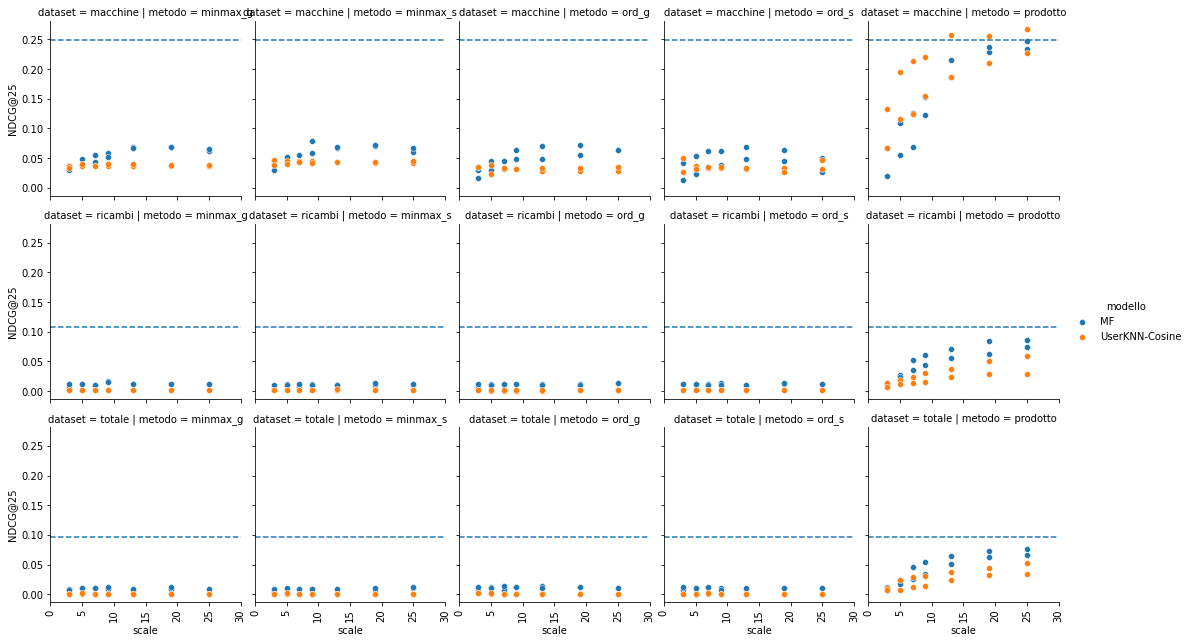
\includegraphics[width=16cm]{figures/comb_1.png}

\subsection{Media matrici dei rating}
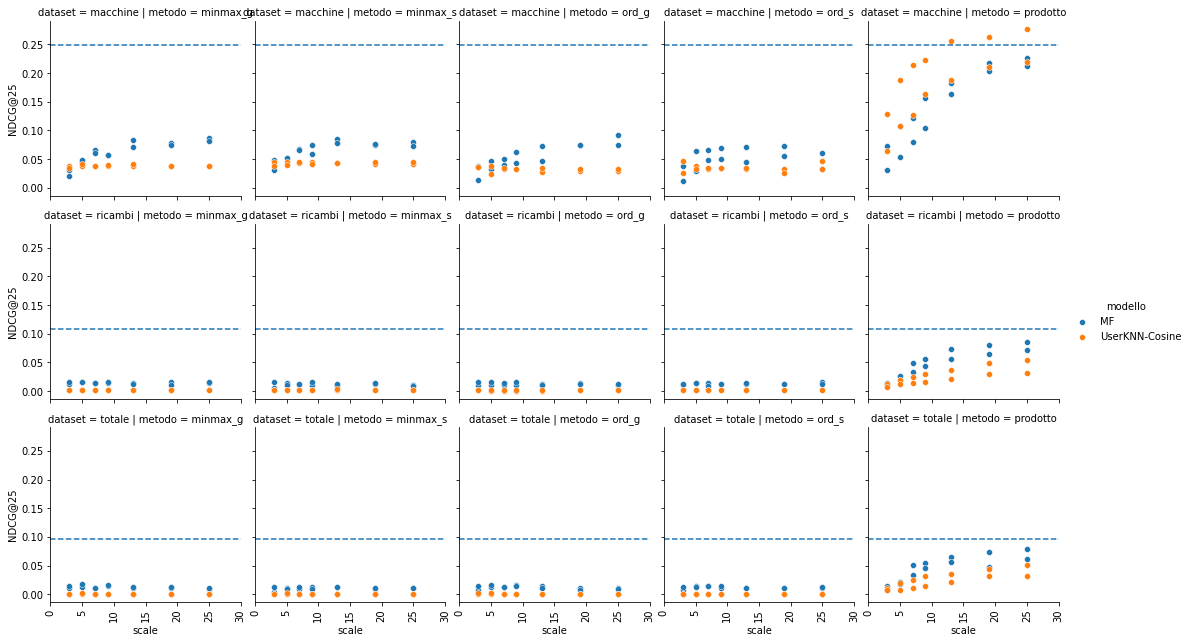
\includegraphics[width=16cm]{figures/comb_2.png}

\section{Esperimenti con approccio next-basket}
In questa sezione vedremo i risultati dell'approccio next-based. Per prima cosa andiamo a vedere quali sono stati i parametri selezionati con il tuning per ciascun dataset.\\

\begin{minipage}[H]{0.45\textwidth}
    \begin{tabular}{|l|ccc|}
        \toprule
        $dataset$ &    $\alpha$ &  $q$ & $r$ \\
        \midrule
        macchine & 0.5 & 100 & $\infty$ \\
        ricambi  &	0.75 & 50 & $\infty$ \\
        totale  & 0 & 100 & $\infty$ \\
    \bottomrule
    \end{tabular}
\end{minipage}
\begin{minipage}[H]{0.55\textwidth}
    Possiamo vedere che alla fine il tuning ha portato ad avere una finestra di recentezza  $r = \infty$, quindi stiamo usando la popolarità \textit{popularity user-wise}. 
\end{minipage}\\

Possiamo inoltre vedere che la località $q$ è comunque alta, mentre per quanto riguarda $alpha$ abbiamo che le macchine calcolano la probabilità composta al 50\%, nei ricambi si da più importanza a quella dello user in esame, ed infine nel totale si considera solo la probabilità composta dello user esterno.

Vediamo i risultati sperimentali con i modelli ottimizzati sul validation set:\\

\begin{tabular}{|l|cccc|}
    \toprule
    $dataset$  &  $NDCG@5$ & $NDCG@10$  & $NDCG@25$ & $NDCG@100$  \\
    \midrule
    macchine & 0.5832 & 0.6278 & 0.6506 & 0.6627 \\
    ricambi & 0.1728 & 0.1892 & 0.2381 & 0.3317 \\
    totale  & 0.2196 & 0.2295 & 0.2834 & 0.3653 \\
\bottomrule
\end{tabular}\\

E ora i corrispondenti risultati con il test set:\\

\begin{tabular}{|l|cccc|}
    \toprule
    $dataset$  &  $NDCG@5$ & $NDCG@10$  & $NDCG@25$ & $NDCG@100$  \\
    \midrule
    macchine & 0.6049 & 0.6476 & 0.6726 & 0.6741 \\
    ricambi & 0.2261 & 0.2403 & 0.2915 & 0.3811 \\
    totale  & 0.1955 & 0.2045 & 0.2595 & 0.3537 \\
\bottomrule
\end{tabular}\\

Ricordiamo che questi risultati non sono confrontabili con quelli delle sezioni precendenti, però i risultati sembrano molti interessanti.